\begin{figure}
\centering
\vspace{-12px}
\subfloat[\textit{First Index} metric]{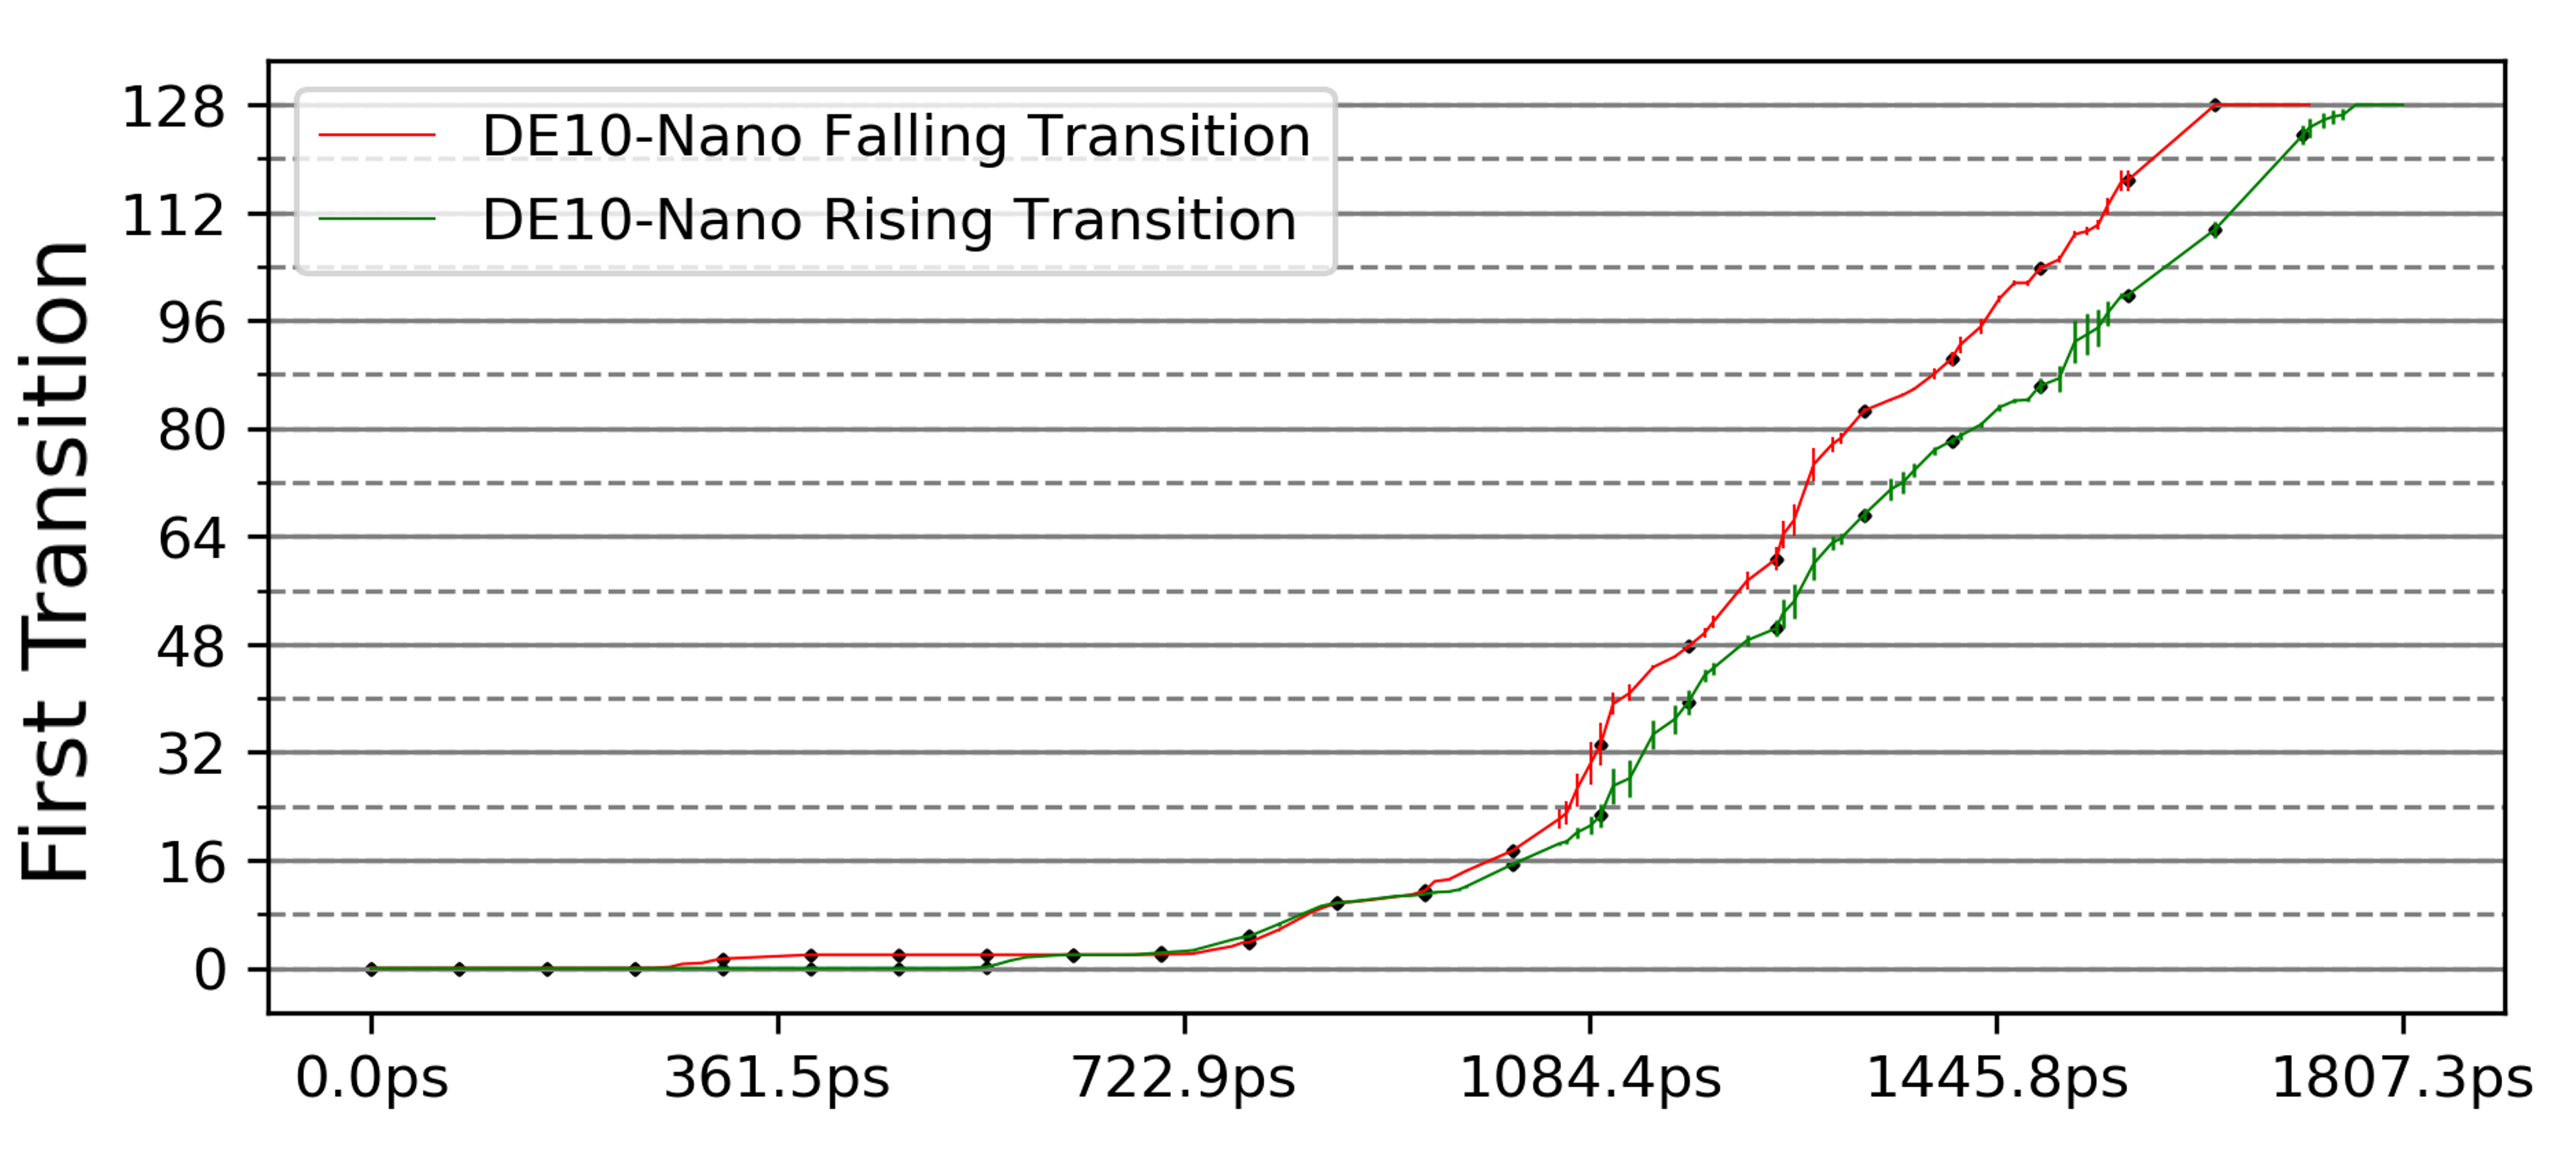
\includegraphics[width= 0.70\linewidth]{img/intel_first.png}\label{fig:prop-first-intel}}\\
\vspace{-12px}
\subfloat[\textit{Last Index} metric]{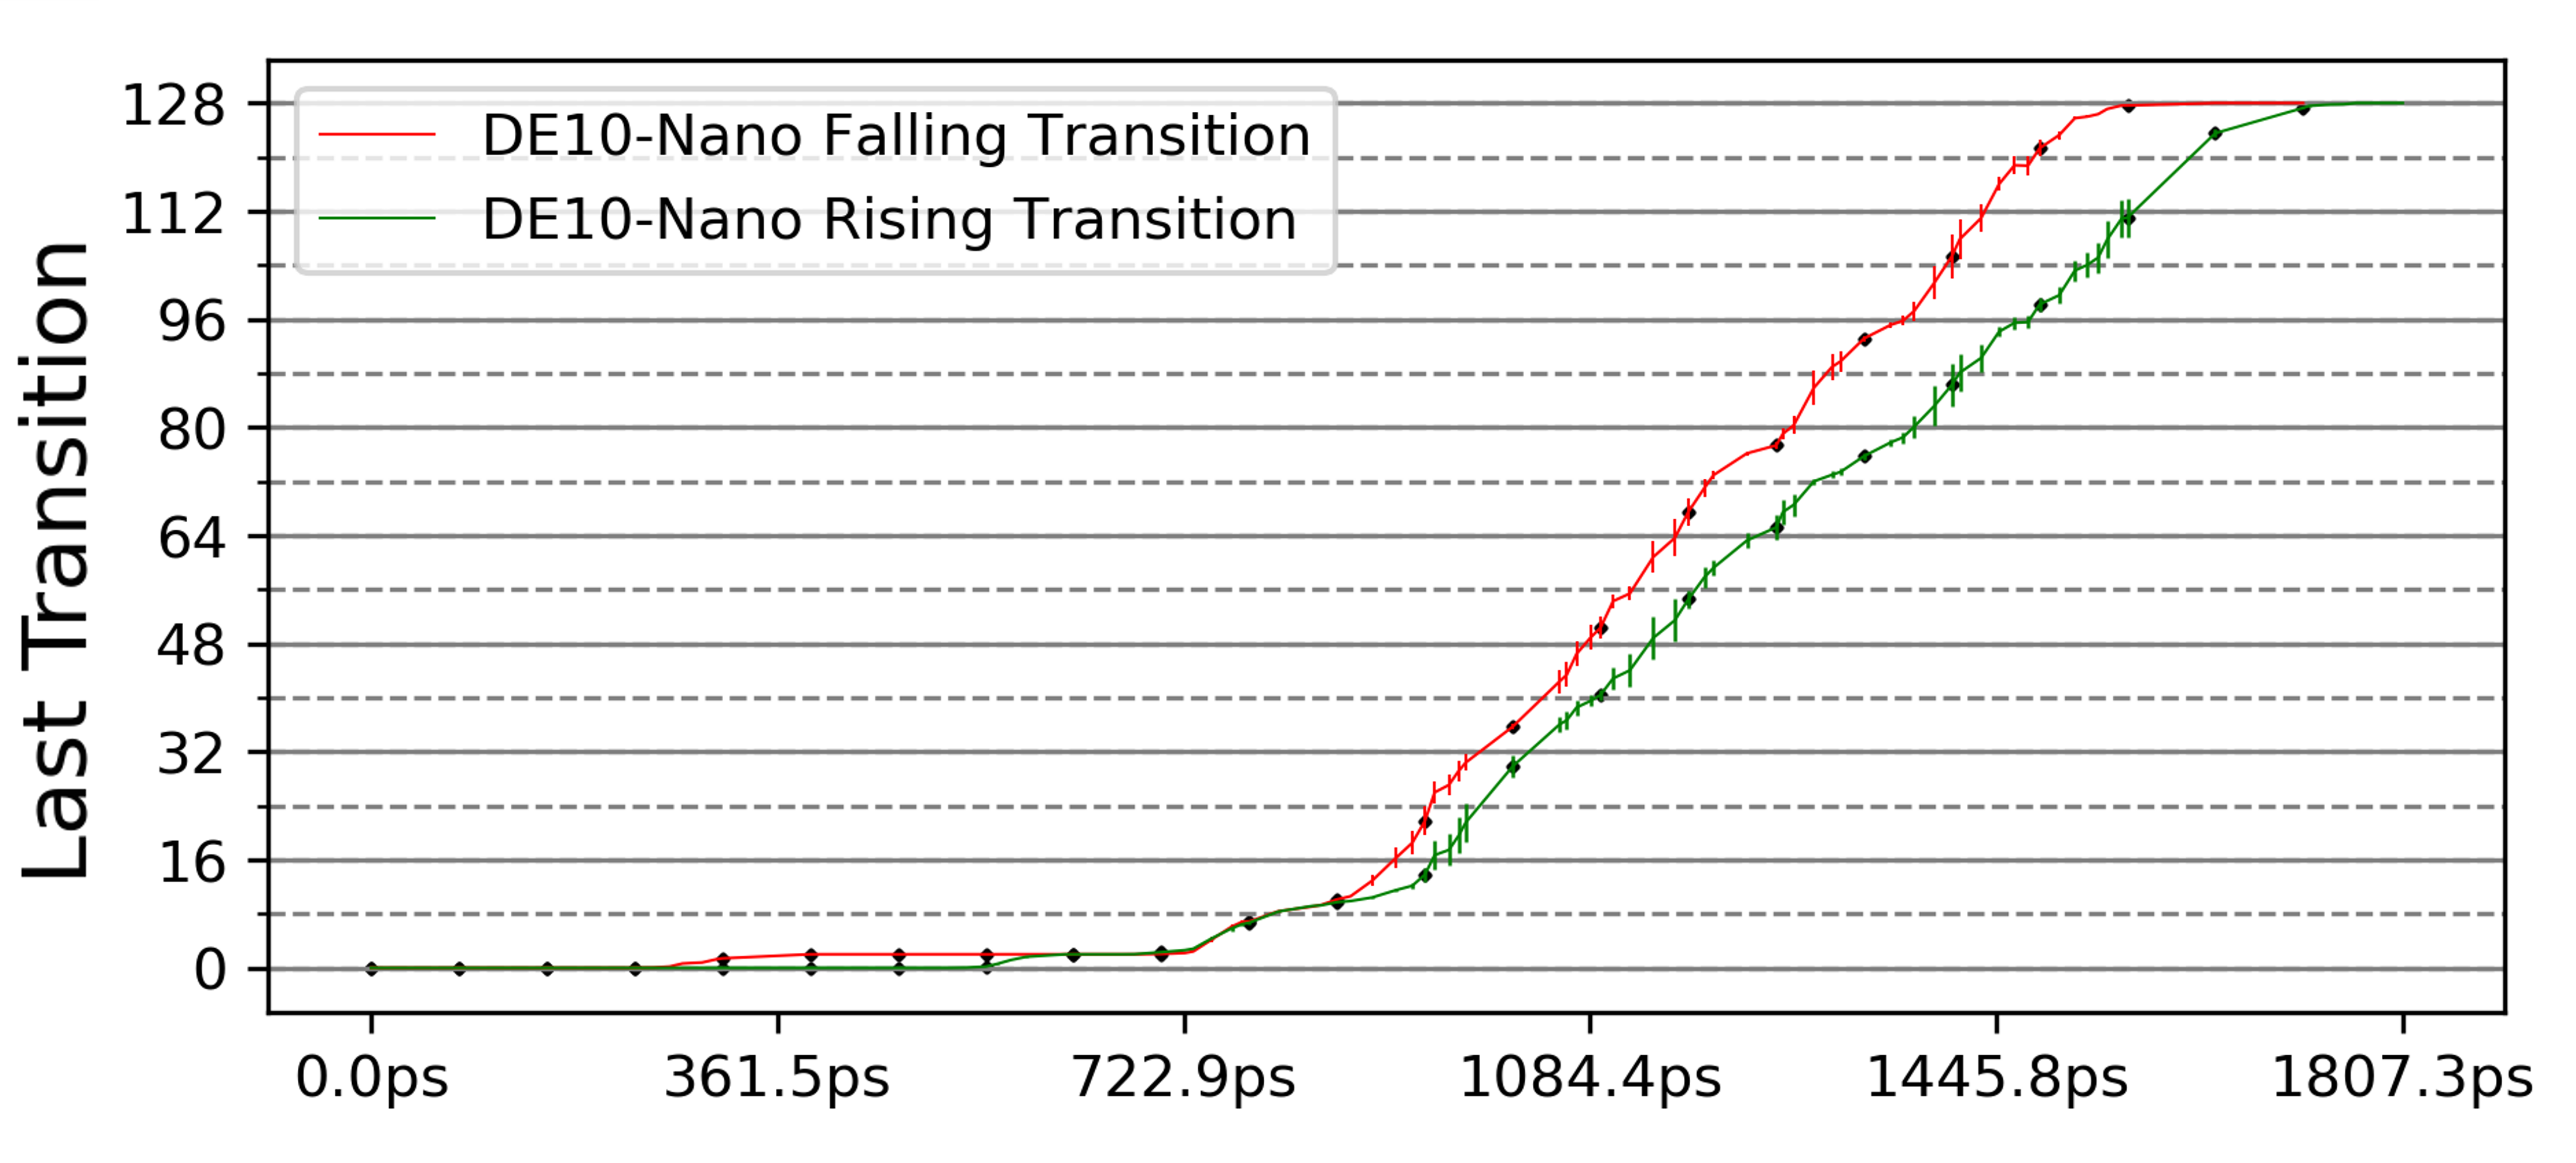
\includegraphics[width= 0.70\linewidth]{img/intel_last.png}\label{fig:prop-last-intel}}\\
\vspace{-12px}
\subfloat[\textit{Binary Hamming Distance} metric]{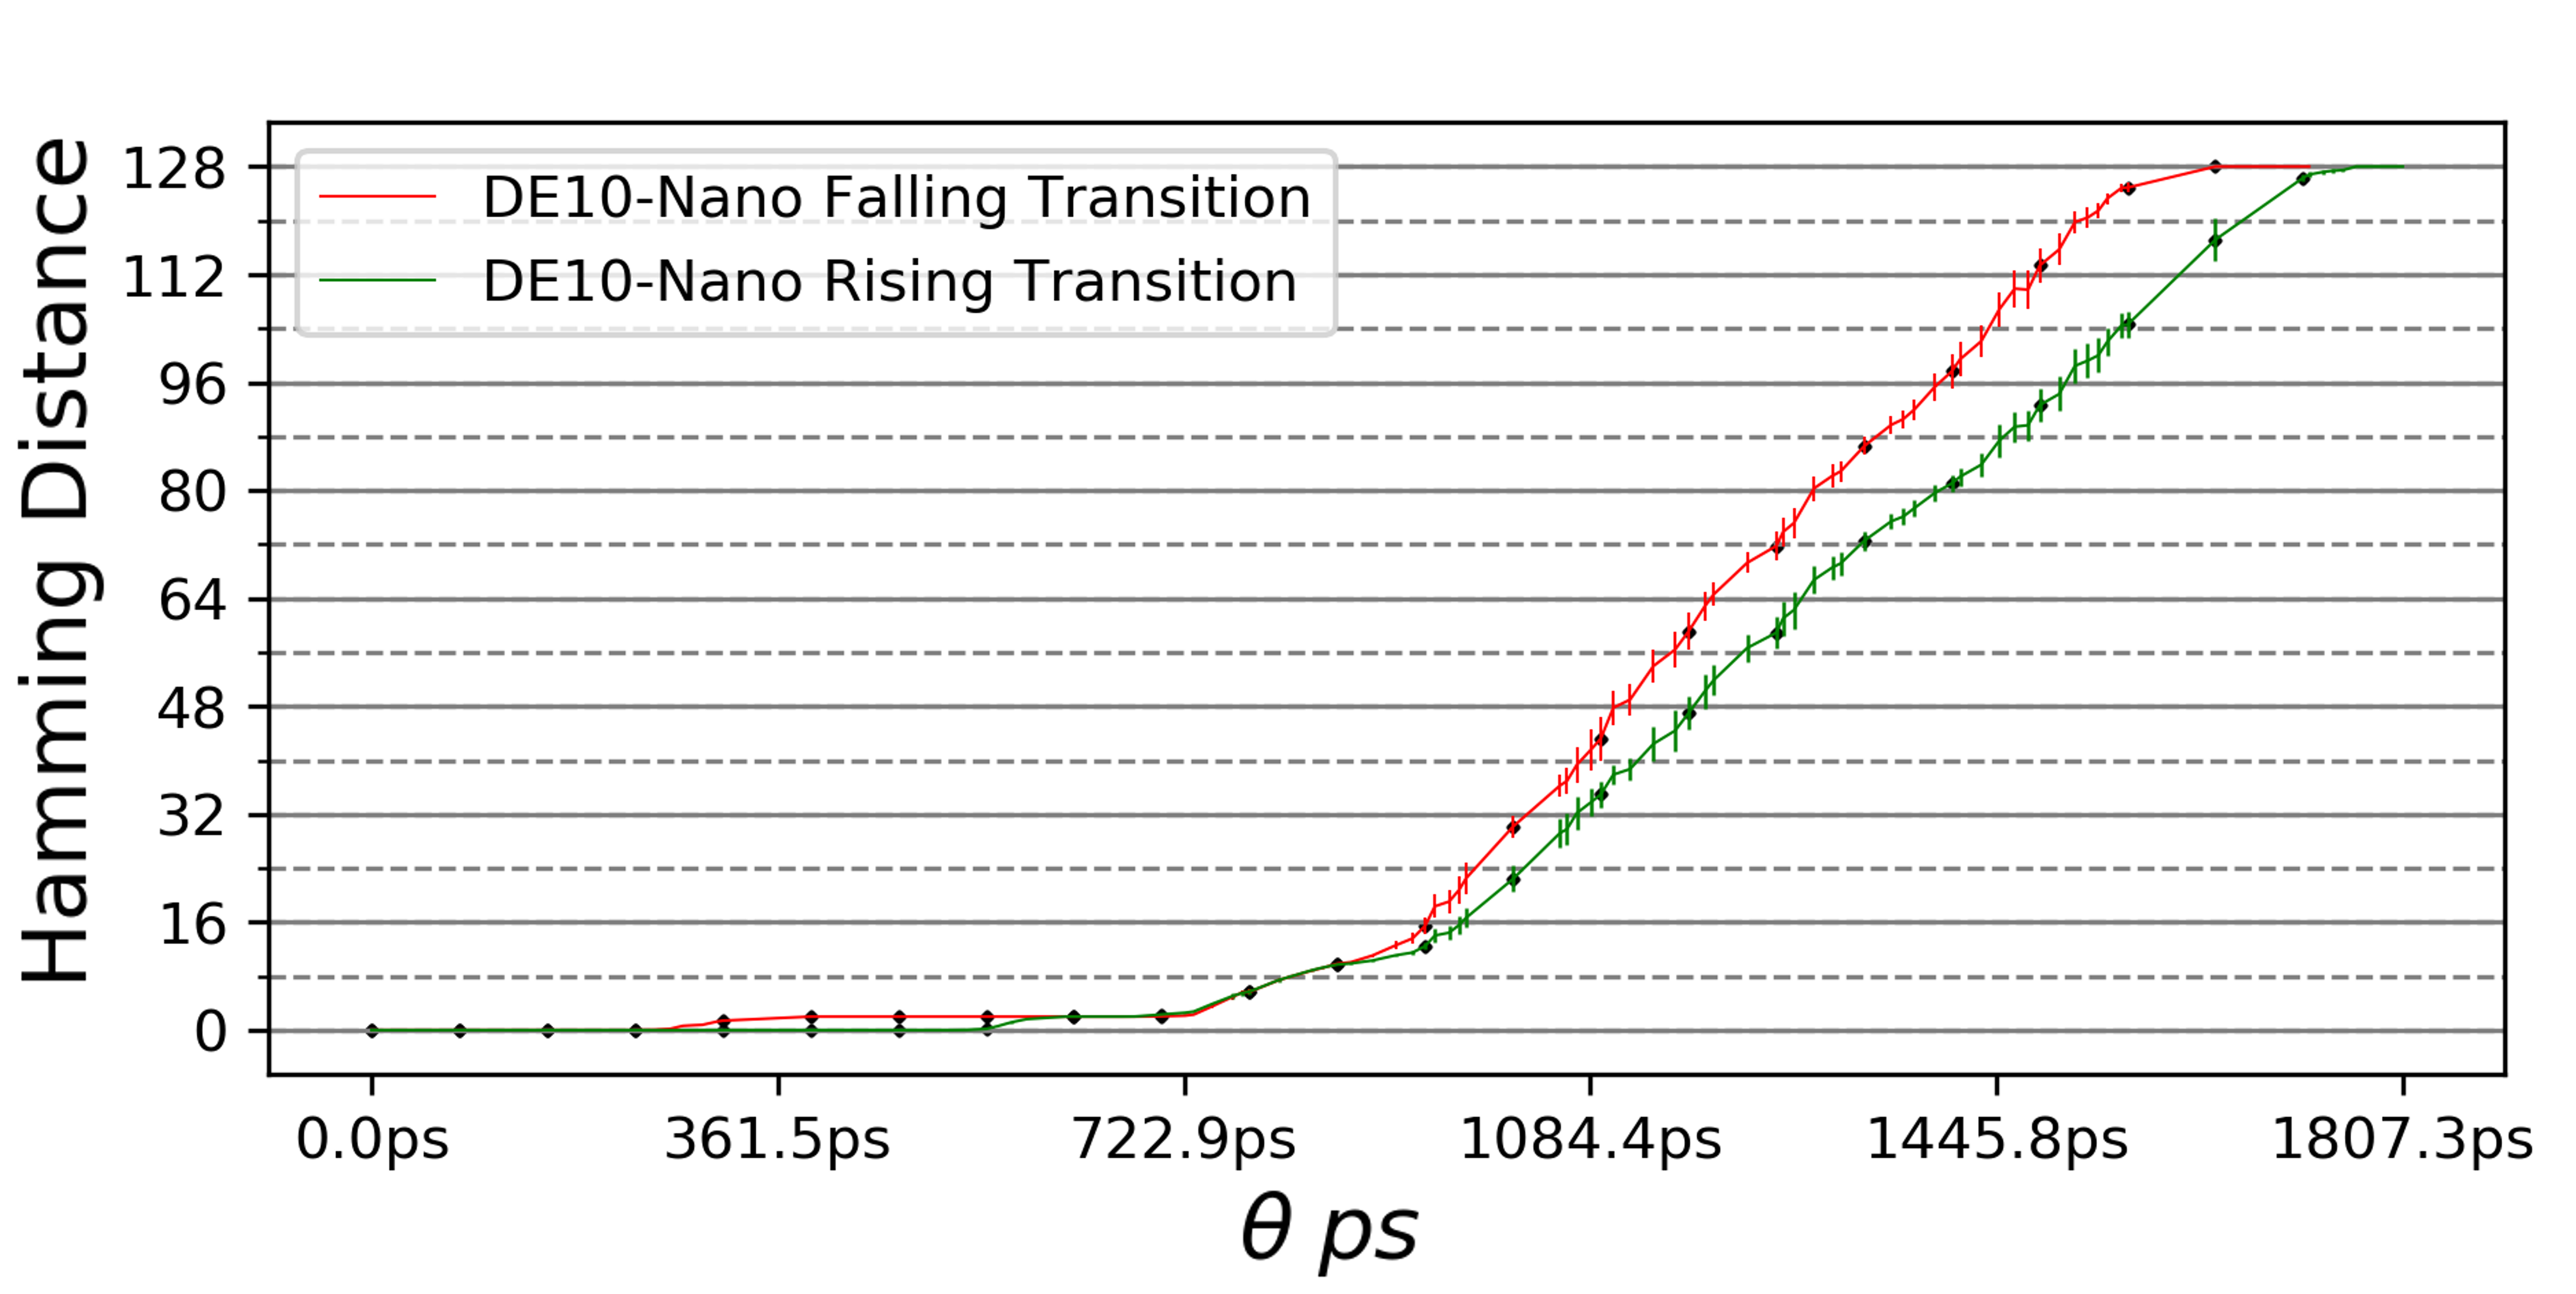
\includegraphics[width= 0.70\linewidth]{img/intel_ham.png}\label{fig:prop-pop-intel}}
\caption{Intel DE10-Nano propagation metrics for both polarities. Non-linearity in the propagation metric does not correspond directly to any known structure within the carry-chain as demonstrated on Xilinx. As demonstrated on Xilinx, hamming weight produces a significantly more linear propagation metric than the first and last transition metrics. The black diamonds represent the worst-case phase step increment and show the improvement in resolution achieved by our PLL configuration prepossessing algorithm.} %\cd{TODO - text bigger maybe. Combine x-axis to just bottom }} 
\label{fig:propagation-intel}
\end{figure}
